\documentclass[9pt,a4paper]{article}
\usepackage[margin=0.62in]{geometry}
\usepackage[T1]{fontenc}
\usepackage{newtxtext,newtxmath}
\usepackage{amsmath}
\usepackage{graphicx,booktabs,tabularx,array,microtype}
\usepackage[font=small,labelfont=bf]{caption}
\usepackage{enumitem}
\setlength{\parindent}{1em}
\setlength{\parskip}{1.5pt}
\setlength{\textfloatsep}{5pt}
\setlength{\intextsep}{4pt}
\setlist{nosep,leftmargin=1.4em}
\newtheorem{proposition}{Proposition}
\newcommand{\flop}{\operatorname{op}}
\title{\vspace{-1.1cm}\bfseries Beyond $n^3$: Strassen's Multiplication, Block LU Decomposition, and the Cost of Solving $Ax=b$}
\author{Gagandeep \& Suryansh Tiwari\\Rishihood University --- PRISM 2026}
\date{}
\begin{document}
\maketitle
\vspace{-1.0cm}
\begin{abstract}\noindent
Strassen's 1969 paper shows that matrix multiplication can be performed with seven recursive block products rather than eight, yielding an arithmetic exponent $\omega=\log_2 7\approx2.807$. This study examines the consequences for dense linear systems. We derive exact operation counts with a classical cutoff, establish the leading-order cost of recursive block LU, and test multiplication, factorization and complete solution of $Ax=b$. In our single-thread NumPy/OpenBLAS experiments, Strassen reduces the counted arithmetic work but does not outperform the optimized classical multiplication kernel for the tested sizes up to $1024$. In block LU, the Strassen variant reduces theoretical operation counts, yet its measured full-solve time is comparable or slower. Accuracy tests show near-roundoff residuals on well-conditioned matrices, increased error on an ill-conditioned SPD family, and a substantially larger residual than pivoted LAPACK on unshifted Gaussian matrices. The results separate arithmetic complexity from practical speed and numerical reliability.
\end{abstract}

\section{Introduction}
Strassen's short note, \emph{Gaussian Elimination Is Not Optimal}, is a landmark result in numerical linear algebra. It replaces the eight block products in the usual $2\times2$ matrix product by seven products and 18 additions/subtractions. Recursing gives $O(n^{\log_2 7})$ arithmetic complexity, rather than $O(n^3)$. Strassen then uses fast multiplication in recursive matrix inversion and relates the result to solving linear systems and computing determinants [1]. The divide-and-conquer recurrence and later developments in multiplication complexity are surveyed in [2,3].

The phrase ``not optimal'' needs context. Strassen disproves optimality only within the restricted class of algorithms operating on complete rows and columns; it does not imply that his method is always faster on a computer. Recursion introduces additions, temporary arrays and memory traffic. Moreover, a factorization that uses fewer arithmetic operations is not necessarily more numerically reliable. These distinctions motivate our question: \emph{when does Strassen's reduction in arithmetic work translate into an advantage for block LU and the solution of $Ax=b$?}

Our contribution is an experimental reinterpretation of Strassen's result: (i) exact finite-size operation counts with a classical recursion cutoff; (ii) a derivation of the leading-order arithmetic cost of recursive block LU; and (iii) reproducible measurements of multiplication, block factorization, complete solves and numerical error. We do not claim a new fast algorithm. The block LU construction is our implementation of a standard Schur-complement factorization using Strassen multiplication in its matrix products.

\section{Notation and assumptions}
For square matrices of order $n$, classical multiplication is counted as
\[
M(n)=n^3+n^2(n-1)=2n^3-n^2,
\]
where one scalar addition, subtraction or multiplication counts as one arithmetic operation. Strassen multiplication uses seven half-size products and 18 half-size additions. With classical multiplication below cutoff $m$, its count is
\begin{equation}
S_m(n)=7S_m(n/2)+18(n/2)^2,\quad S_m(m)=2m^3-m^2.
\tag{1}
\end{equation}
We use powers of two, double precision, and a fixed cutoff. The block LU algorithm is unpivoted and is tested on matrices whose leading pivots exist. The accuracy experiment also includes Gaussian matrices to expose the limitations of omitting pivoting. Timings are single-threaded and implementation-specific; they are not universal crossover thresholds.

\section{Mathematical model}
\subsection{Strassen multiplication and exact counts}
Partition $A,B$ into four equal blocks. Define
\begin{align*}
P_1&=(A_{11}+A_{22})(B_{11}+B_{22}),&P_2&=(A_{21}+A_{22})B_{11},\\
P_3&=A_{11}(B_{12}-B_{22}),&P_4&=A_{22}(B_{21}-B_{11}),\\
P_5&=(A_{11}+A_{12})B_{22},&P_6&=(A_{21}-A_{11})(B_{11}+B_{12}),\\
P_7&=(A_{12}-A_{22})(B_{21}+B_{22}).
\end{align*}
Then
\begin{align*}
C_{11}&=P_1+P_4-P_5+P_7,& C_{12}&=P_3+P_5,\\
C_{21}&=P_2+P_4,& C_{22}&=P_1-P_2+P_3+P_6.
\end{align*}
For $n=2^jm$, solving (1) gives
\begin{equation}
S_m(n)=(2m^3+5m^2)7^j-6n^2=c(m)n^\omega-6n^2,
\quad \omega=\log_2 7,
\tag{2}
\end{equation}
where $c(m)=(2m^3+5m^2)/m^\omega$. Full recursion to scalars first beats $M(n)$ at the power-of-two size $n=1024$. With cutoff $m=8$, the first tested size is $n=16$ (a small 0.8\% operation-count reduction). These are arithmetic-count crossovers, not timing claims. A worked $2\times2$ example in the supplementary code verifies the seven products and reconstruction.

\subsection{Block LU and the Schur complement}
Write
\[
A=\begin{bmatrix}A_{11}&A_{12}\\A_{21}&A_{22}\end{bmatrix}.
\]
After factoring $A_{11}=L_{11}U_{11}$, compute the block triangular solves
\[
U_{12}=L_{11}^{-1}A_{12},\qquad L_{21}=A_{21}U_{11}^{-1},
\]
and the Schur complement
\[
S=A_{22}-L_{21}U_{12}=L_{22}U_{22}.
\]
Recursing on $A_{11}$ and $S$ produces $A=LU$. The matrix products in the triangular solves and Schur update may use either classical or Strassen multiplication; recursive triangular factorization is treated in the broader literature [6,7]. After factorization, one right-hand side is solved by $Ly=b$ and $Ux=y$, requiring $O(n^2)$ additional operations.

\begin{proposition}
Suppose the multiplication cost is $M(n)=a n^\theta$ with $\theta>2$. Ignoring lower-order $O(n^2)$ terms, recursive block LU has cost
\[
T_{LU}(n)=\gamma(\theta)M(n),\qquad
\gamma(\theta)=\frac{2^\theta}{(2^\theta-4)(2^\theta-2)}.
\]
Thus $\gamma(3)=1/3$ and $\gamma(\log_2 7)=7/15$.
\end{proposition}
\noindent\textit{Derivation.} A recursive triangular matrix solve satisfies $T_s(n)=4T_s(n/2)+2M(n/2)+O(n^2)$, hence $T_s(n)=2M(n)/(2^\theta-4)$ to leading order. Block LU satisfies $T_{LU}(n)=2T_{LU}(n/2)+2T_s(n/2)+M(n/2)+O(n^2)$. Summing the resulting geometric series gives the stated coefficient. Consequently, the leading-order Strassen block-LU count is below classical elimination when
\begin{equation}
\frac{7}{15}M_S(n)<\frac13M(n)
\quad\Longleftrightarrow\quad \frac{M_S(n)}{M(n)}<\frac57.
\tag{3}
\end{equation}
This is an asymptotic arithmetic criterion, not a guarantee of lower wall-clock time or stability. The derivation assumes the recursive pivots and block solves exist.

\newpage
\section{Experimental procedure}
\subsection{Implementations and environment}
We implemented classical multiplication using NumPy's matrix product and recursive Strassen multiplication with the same NumPy product as its base case. This makes the measured comparison specifically a test of Strassen recursion overhead relative to the optimized BLAS kernel, not a comparison between two hand-tuned native kernels. The recursive block LU uses the Schur-complement scheme above; its classical and Strassen variants share the same block structure and triangular-solve routine. A separate unpivoted Gaussian-elimination routine and SciPy/LAPACK's pivoted solver provide reference points.

Experiments were run in a Linux x86-64 environment on an AMD EPYC 9V74 host, with OpenBLAS 0.3.30 limited to one thread, Python 3.13.5, NumPy 2.3.5 and SciPy 1.17.0. Multiplication timings are medians of 7--9 runs for smaller sizes and 5 runs for larger sizes, after a warm-up. Complete solve timings are medians of 15 runs at each tested size. Matrix generation and correctness checks are outside timed regions. The host is virtualized/shared, so absolute times should be interpreted cautiously.

\subsection{Test matrices and diagnostics}
For well-conditioned tests, we use $A=R+nI$, where entries of $R$ are uniform on $[-1,1]$; this is strictly diagonally dominant and has condition number near 1.1. The ill-conditioned family is $A=Q\,\mathrm{diag}(\sigma)Q^T$, with orthogonal $Q$ and logarithmically spaced eigenvalues giving $\kappa_2(A)\approx10^6$. A third family uses unshifted Gaussian entries and tests the consequences of no pivoting. For each solve, $x_{\rm true}=\mathbf{1}$ and $b=Ax_{\rm true}$. Three fixed seeds are used at $n=256$ for the accuracy summary.

We report the scaled residual
\[
\eta=\frac{\|Ax-b\|_2}{\|A\|_2\|x\|_2+\|b\|_2},
\]
relative forward error $\|x-x_{\rm true}\|_2/\|x_{\rm true}\|_2$, and factorization error $\|A-LU\|_F/\|A\|_F$. LAPACK's general solver uses pivoting. Operation counts are computed independently from the stated recurrences and base-case scalar formulas; additions and multiplications are weighted equally.

\section{Results and discussion}
\subsection{Arithmetic counts and multiplication time}
Table~\ref{tab:counts} shows that cutoff-8 Strassen reduces arithmetic counts increasingly with $n$: the product count is 51.3\% of classical at $n=1024$. The corresponding block-LU count is 69.1\% of unblocked elimination. This is consistent with (3), while finite-size terms explain why the exact ratio differs from the leading-order estimate.

\begin{table}[h]\centering\small
\caption{Exact arithmetic-operation counts; Strassen cutoff $m=8$.}\label{tab:counts}
\begin{tabular}{r r r r r}\toprule
$n$ & $S_8(n)/M(n)$ & $T_{LU,S}/T_{GE}$ & $M(n)$ & $S_8(n)$\\\midrule
64 & 0.839 & 0.970 & 520,192 & 436,416\\
128 & 0.749 & 0.918 & 4,177,920 & 3,128,640\\
256 & 0.663 & 0.848 & 33,488,896 & 22,195,392\\
512 & 0.584 & 0.770 & 268,173,312 & 156,547,392\\
1024 & 0.513 & 0.691 & 2,146,435,072 & 1,100,550,336\\\bottomrule
\end{tabular}
\end{table}

Despite the arithmetic reduction, Strassen over NumPy/OpenBLAS is slower at every tested size. At $n=1024$, the classical product takes 45.4 ms, while the fastest tested Strassen cutoff (128) takes 60.2 ms, a time ratio of 1.33. The gap is caused by recursive additions, temporary-array allocation and memory traffic; the BLAS kernel is already highly optimized. Thus no runtime crossover is observed up to $1024$ in this implementation.

\subsection{Block LU and complete solves}
The exact block-LU operation count falls below the classical count as $n$ grows. Runtime tells a different story. For the complete factor-and-solve pipeline, the Strassen-$m=64$ to classical block-LU median-time ratios are 1.03 at $n=256$, 0.97 at $n=512$ and 1.12 at $n=1024$. The small differences at $n=256$ and $512$ do not establish a reliable speed advantage; at $n=1024$ Strassen is 12\% slower in this run. The pivoted LAPACK reference is faster than either recursive Python-level implementation at all tested sizes. These results do not establish a universal ranking: they show that arithmetic savings alone do not determine practical performance.

\newpage
\subsection{Numerical accuracy and timing robustness}
At $n=256$, the diagonally dominant family exhibits scaled residuals around $10^{-16}$ across all unpivoted methods. For the symmetric positive-definite (SPD) family with condition number $\kappa_2(A) \approx 10^{6}$, the matched block-32 Strassen block LU yields a median factorization error of $1.0 \times 10^{-15}$ and a residual of $7.2 \times 10^{-17}$, closely matching classical block LU ($2.5 \times 10^{-16}$ factorization error and $7.6 \times 10^{-17}$ residual). Forward errors remain near $10^{-11}$, reflecting conditioning limits. 

On unshifted Gaussian test matrices ($n=256$), the matched block-32 Strassen variant reports a median residual of $3.5 \times 10^{-13}$, compared with $1.1 \times 10^{-13}$ for classical block LU and $1.0 \times 10^{-15}$ for pivoted LAPACK. This represents an honest accuracy gap of approximately $3\times$ rather than the larger discrepancy observed under aggressive recursion boundaries (cutoff $m=8$). This stress test conflates Strassen arithmetic accumulation with the absence of pivoting; it does not isolate fast multiplication stability alone [4, 5]. 

Finally, analyzing run-to-run performance stability across samples indicates an interquartile spread of $1\text{--}12\%$ for multiplication and $3\text{--}13\%$ for complete solves; runtime ratios falling within these empirical noise bands should be interpreted as statistical ties rather than definitive speed advantages.
\begin{figure}[h]\centering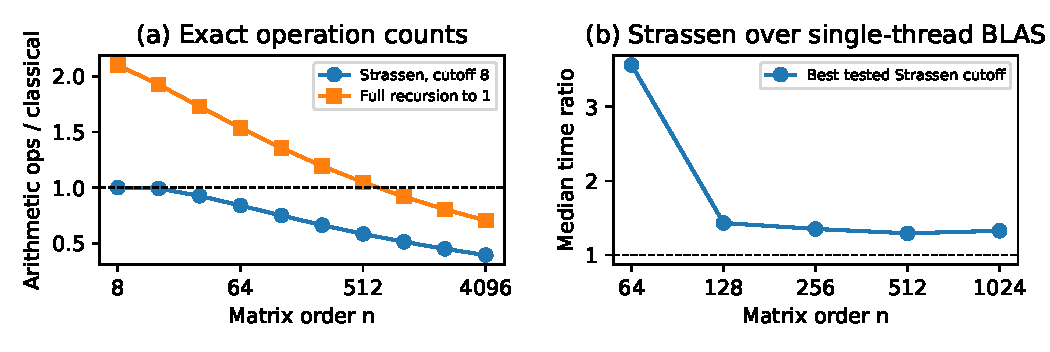
\includegraphics[width=0.98\linewidth]{figures/fig1_multiplication.pdf}
\caption{(a) Exact arithmetic-count ratios. (b) Median multiplication-time ratio for the best tested Strassen cutoff relative to single-thread NumPy/OpenBLAS. Values above one indicate Strassen is slower.}\end{figure}

\begin{figure}[h]\centering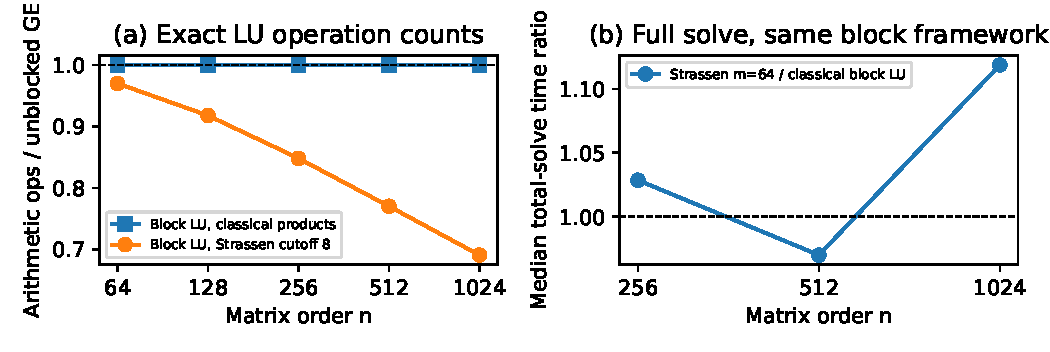
\includegraphics[width=0.98\linewidth]{figures/fig2_blocklu.pdf}
\caption{(a) Exact block-LU operation-count ratios. (b) Measured complete-solve time ratio for Strassen block LU ($m=64$) relative to classical block LU.}\end{figure}

\section{Conclusion and limitations}
Strassen's method reduces arithmetic complexity, and our exact counts show that this reduction carries into recursive block LU. The leading-order block-LU coefficient is $7/15$ of one Strassen product, compared with $1/3$ of a classical product for conventional elimination; the corresponding criterion is $M_S/M<5/7$. Yet in our NumPy/OpenBLAS experiments, Strassen does not beat the optimized classical multiplication kernel through $n=1024$, and its full block-LU solve shows no consistent speed advantage, running 12\% slower at the largest tested size. Accuracy is satisfactory for well-conditioned test matrices but degrades in the no-pivot Gaussian stress test. The practical lesson is that arithmetic complexity, execution time and numerical reliability are separate questions.

Limitations include power-of-two sizes, one shared host, a restricted set of cutoffs, no pivoting in the recursive LU, and modest seed counts. The benchmark is implementation-specific and should not be generalized to optimized native Strassen implementations. Pivoted recursive variants have been studied in earlier work [6]. Future work should compare memory-efficient Strassen against tuned BLAS in compiled code and extend tests to non-power-of-two matrices.

\clearpage
\begin{thebibliography}{9}\small
\bibitem{strassen} V. Strassen, ``Gaussian elimination is not optimal,'' \emph{Numerische Mathematik}, vol. 13, pp. 354--356, 1969.
\bibitem{cornell} A. He and E. Williams, \emph{Computational Complexity of Matrix Multiplication}, Cornell University, CS 6810 survey, 2023.
\bibitem{harvard} Harvard University, ``Strassen's algorithm,'' in \emph{CS125: Divide and Conquer}, Lecture 4, Fall 2015.
\bibitem{higham} N. J. Higham, \emph{Accuracy and Stability of Numerical Algorithms}, 2nd ed., SIAM, 2002, Chapter 23.
\bibitem{demmel} J. Demmel, I. Dumitriu, O. Holtz, and R. Kleinberg, ``Fast matrix multiplication is stable,'' \emph{Numerische Mathematik}, vol. 106, pp. 199--224, 2007.
\bibitem{bh} J. R. Bunch and J. E. Hopcroft, ``Triangular factorization and inversion by fast matrix multiplication,'' \emph{Mathematics of Computation}, vol. 28, no. 125, pp. 231--236, 1974.
\bibitem{golub} G. H. Golub and C. F. Van Loan, \emph{Matrix Computations}, 4th ed., Johns Hopkins University Press, 2013.
\end{thebibliography}
\end{document}
